\chapter{Results and Analysis}
\label{chapter:results}

\section{Hot Paths}

The following sections analyzes the submissions to the \gls{nist} standardization process, in terms of the reference implementations and what branches the code takes, how many times they are taken\footnote{In applicable cases}, as well as how many instructions is spent in a function. Unless otherwise stated, the measurements are the percentage of instructions performed in a function or in a line of code, relative to the parent. 

All of the data as well as further visualizations not included in this work is published on GitHub\footnote{\href{https://github.com/profiling-pqc-kem-thesis/data}{https://github.com/profiling-pqc-kem-thesis/data}}.

\subsection{NTRU}

The \gls{ntru} reference implementations consists of three API methods - keypair generation via \textit{crypto\_kem\_keypair}, encryption (encapsulation) via \textit{crypto\_kem\_enc} and decryption (decapsulation) via \textit{crypto\_kem\_dec}  decryption (decapsulation). These API functions may in turn call several internal functions, such as the polynomial math library which functions are prefixed \textit{poly\_}.

The following graphs contain relative measurements denoting the percentage of instructions spent in each method. Both the HPS and HRSS variants of \gls{ntru} perform alike, hence only one set of graphs is shown for \gls{ntru} as a whole.

Figure \ref{figure:result:hot-paths:ntru:crypto_kem_keypair} shows us that $40\%$ of the instructions of generating a key-pair is spent in the library function \textit{poly\_Rq\_mul} - a function which multiplies two polynomials in $\mathbb{R}^q$. Another $20\%$ of the instructions are spent on inverting a polynomial in $\mathbb{R}^2$ - in \textit{poly\_R2\_inv}. In total, the polynomial math accounts for at least $60\%$ of the time spent on generating a keypair.

\begin{figure}[H]
    \centering
    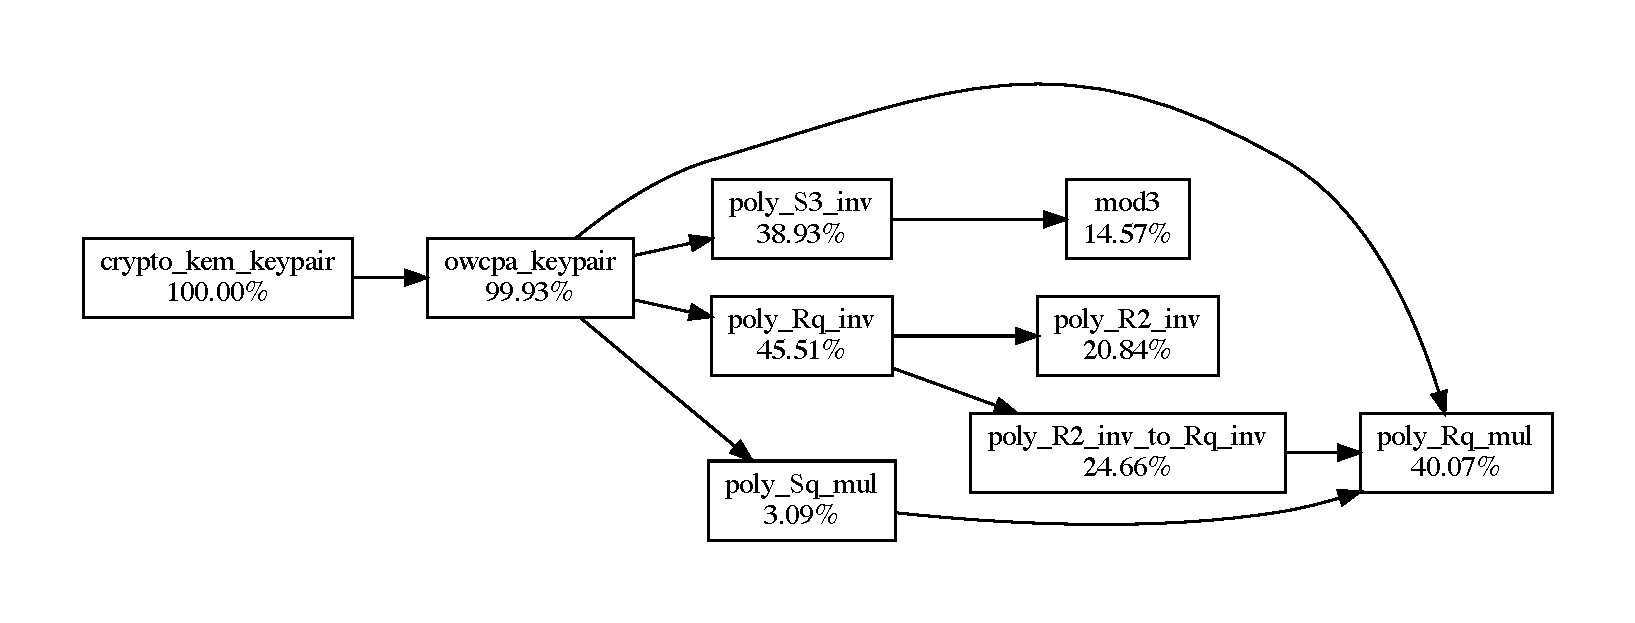
\includegraphics[width=15cm, height=10cm, keepaspectratio]{chapters/results/hot-paths/ntru/crypto_kem_keypair.pdf}
    \caption{Relative instruction count of \gls{ntru}'s \textit{crypto\_kem\_keypair}}
    \label{figure:result:hot-paths:ntru:crypto_kem_keypair}
\end{figure}

Figure \ref{figure:result:hot-paths:ntru:crypto_kem_enc} describes the encapsulation API function. The key is generated using random bytes which are fed through 256-bit \gls{aes} in its Electronic Code Book (ECB) configuration to produce uniformly random bytes. Again, we see a significant percentage of the instructions spent in the polynomial library - in \textit{poly\_Rq\_mul}.

\begin{figure}[H]
    \centering
    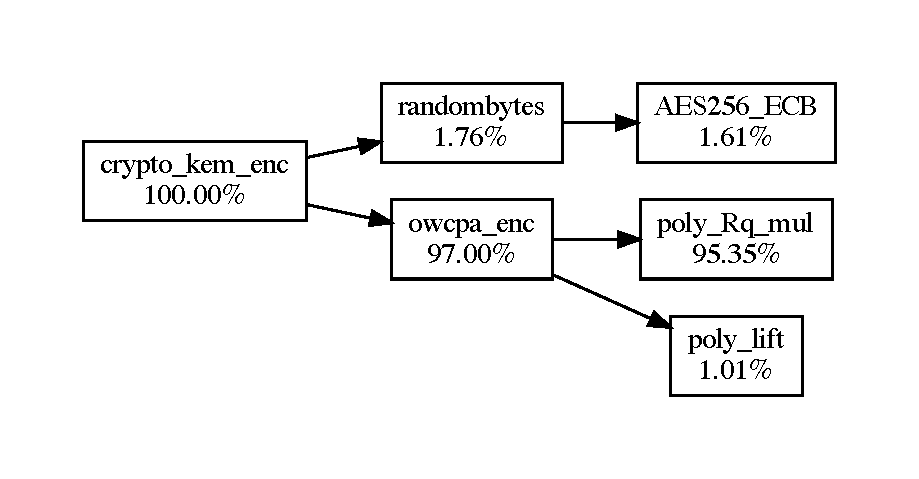
\includegraphics[width=15cm, height=10cm, keepaspectratio]{chapters/results/hot-paths/ntru/crypto_kem_enc.pdf}
    \caption{Relative instruction count of \gls{ntru}'s \textit{crypto\_kem\_keypair}}
    \label{figure:result:hot-paths:ntru:crypto_kem_enc}
\end{figure}

The decryption function of \gls{ntru} is presented in figure \ref{figure:result:hot-paths:ntru:crypto_kem_dec}. Virtually all of the instructions spent decrypting (decapsulating) a key is spent in the \textit{poly\_Rq\_mul} function.

\begin{figure}[H]
    \centering
    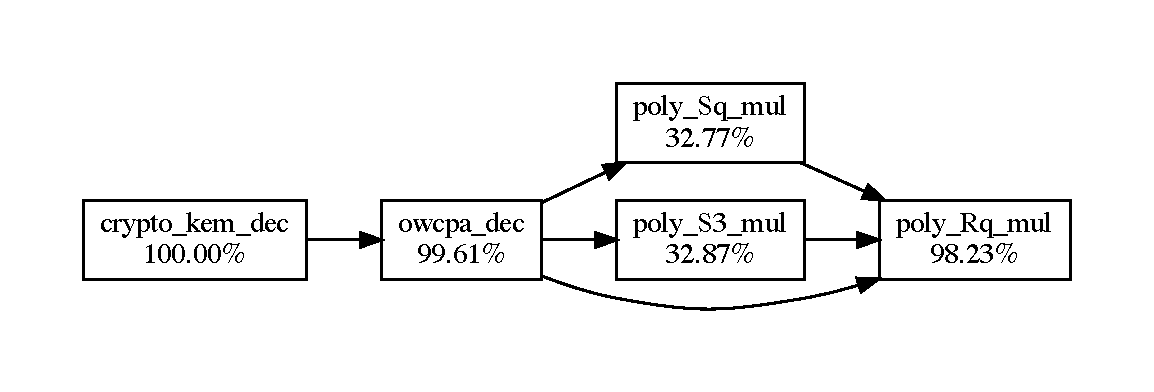
\includegraphics[width=15cm, height=10cm, keepaspectratio]{chapters/results/hot-paths/ntru/crypto_kem_dec.pdf}
    \caption{Relative instruction count of \gls{ntru}'s \textit{crypto\_kem\_dec}}
    \label{figure:result:hot-paths:ntru:crypto_kem_dec}
\end{figure}

Looking at the code of \textit{poly\_Rq\_mul} as shown in figure \ref{figure:result:hot-paths:ntru:poly_Rq_mul}, it is evident that the vast majority of instructions are spent on multiplying and adding numbers in loops. The value of \textit{NTRU\_N} corresponds to the parameter set. For \gls{ntru} HRSS 701, the value is 701 and for \gls{ntru} HPS 4096821 the value is 821.

\begin{figure}[H]
    \centering
    \begin{lstlisting}[language=C]
void poly_Rq_mul(poly *r, const poly *a, const poly *b) {
  int k, i;

  for (k = 0; k < NTRU_N; k++) {
    r->coeffs[k] = 0;
    for (i = 1; i < NTRU_N - k; i++) // 10.21%
      r->coeffs[k] += a->coeffs[k + i] * b->coeffs[NTRU_N - i]; // 42.75%
    for (i = 0; i < k + 1; i++) // 8.20%
      r->coeffs[k] += a->coeffs[k - i] * b->coeffs[i]; // 38.79%
  }
}
    \end{lstlisting}
    \caption{Annotated source code of NTRU's \textit{poly\_Rq\_mul}}
    \label{figure:result:hot-paths:ntru:poly_Rq_mul}
\end{figure}

To summarize, it is shown that factors such as the speed of \gls{aes} has little to do with the overall performance of the algorithm. Furthermore, it seems as if the polynomial library functions account for the vast majority of instructions spent on key-pair generation, encryption and decryption. The function \textit{poly\_Rq\_mul}, which multiplies two polynomials in $\mathbb{R}^q$), accounts for most of the calculations performed.

\todo[inline]{Förtydliga varför vi inte egentligen använder hot paths här? Det är ju bara tid per funktion - inte hur ofta branches tas.}

\subsection{Classic McEliece}
The \gls{mceliece} reference implementation consists of three API methods - \textit{crypto\_kem\_keypair}, \textit{crypto\_kem\_enc} and \textit{crypto\_kem\_dec} for key-pair generation, encryption (encapsulation) and decryption (decapsulation), respectively. These API functions may in turn call several internal functions, such as the \textit{pk\_gen} function that takes up most of the execution time. 

\todo[inline]{Var tydliga med hot paths och tid. Exempelvis så lär diagrammet för pk\_gen visa 0\% för vissa funktioner så som root, men om vi ser till hot paths så lär vi se att de kallas flera miljoner gånger. Kanske ha en graf som visar antalet invocations?}